\subsection{How Developers Develop Features\\ \textit{T. Girba, O. Greevy, S. Ducasse (CSMR'2007)}}

In 2007 the same team published this paper\cite{Girba2007}, on a similar subject as the previous. This time, they shifted their focus towards ownership of features as well as files. Indeed, the regular point of view, ownership of packages, is how the developpers think about their code, however domain analysists and users are more likely thinking in terms of features. Analysing this metric could be usefull to link the external perspective of a project and its internal structure.
The visualisation displays the ownership of files within the projects features, which are also structurally linked. The following image is a representation of this visualisation on a program that is designed to manage a mobile phone:

\begin{figure}[H]
\centering
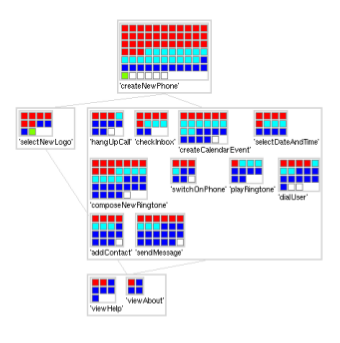
\includegraphics[width=0.4\textwidth]{./resources/girba2007.png}~
\caption{Ownership map By Feature}
\label{fig:ownership_map_by_feature}
\end{figure}

This visualisation makes it possible to determine whom one might ask in order to help resolve a bug in a feature, rather than having to identify which file belong to which feature as one would need to do with the previous paper's visualisation
The goal was also to determine if developpers tend to developp features or functionnal blocks. They saw that projects contributions were mainly distributed on a package boundary.~\ref{fig:annex_ownership_outsight}.
